\documentclass[12pt,a4paper,UTF8]{ctexart}




%设置页边距
\usepackage{geometry}
\geometry{left=2.5cm,right=2.5cm,top=2.5cm,bottom=2.5cm}
\usepackage{wrapfig}



%需要用到的扩展包
\usepackage{xeCJK,amsmath,paralist,enumerate,booktabs,multirow,graphicx,float,subfig,setspace,listings,lastpage,hyperref}
\usepackage{fancyhdr}




%设置页眉页脚以及页码
\pagestyle{fancy}
\rhead{直流单臂电桥}
\lhead{大学基础物理实验报告}
\cfoot{Page\thepage/\pageref{LastPage}}
\rfoot{\today}




%报告中用到的图片存放在这个tex文件所在目录中的figures子目录中
\graphicspath{{figures/}}









%报告开始
\begin{document}
	
	
	
	
	%设置课程标题
	\begin{center}
		\heiti\LARGE{《大学基础物理实验》课程实验报告}
	\end{center}
	
	
	
	
	%设置实验人信息以及实验时间表格
	
	
	\begin{center}
		\begin{tabular}{lcr}
			
			{\songti 姓名及学号:蒋丰毅2211082}  \quad 专业:工科试验班 \quad 年级:22级 \quad 座号:10\\
			{\songti  学院:软件学院 \quad 实验组别:C组\quad 实验时间:2023年4月6日~星期五~上午}\\
			
			
		\end{tabular}
	\end{center}
	\vspace{-0.2cm}
	{\noindent}	 \rule[-10pt]{17.5cm}{0.05em}\\
	
	\vspace{-0.4cm}
	
	
	
	
	
	
	%实验题目
	\begin{center}
		\LARGE\textbf{直流单臂电桥}
	\end{center}
	
	
	
	%实验原理
	\subsection*{[实验原理]}
	

\par
	\begin{figure}[!htbp]
	\centering
	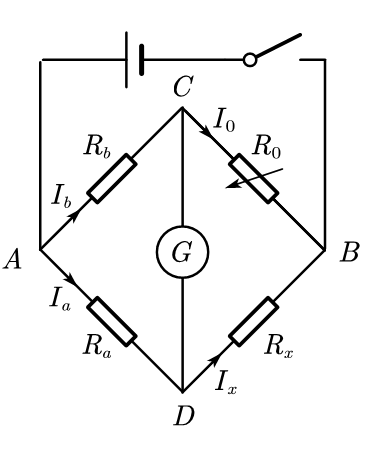
\includegraphics[width=0.3\textwidth]{直流单臂}
	\caption{\footnotesize 实验原理图}
\end{figure}
直流单臂电桥的原理电路如图1所示。它是由四个电阻$R_a,R_b,R_0,R_x$联成一个四边形回路,适当调节$R_0$值,使得$C,D$两点之间无电流通过,这时有:

$$R_aI_a=R_bI_b$$

$$R_xI_x=R_0I_0$$

\par 并且有

$$I_a=I_x,\quad I_b=I_0$$

\par 上式可整理得:

\[R_x=\frac{R_a}{R_b}R_0\]

\par 其中$C=R_a/R_b$,则$R_x=CR_0$
\clearpage
\par 支流双臂电桥适用于测量中等阻值($10\sim 10^5\Omega$),对于比例臂倍率$C$的选取, 应选取倍率$C$使得$R_0$调节的有效位数更多,即应使得$R_X/C$的大致值需要用电阻箱的每一个旋钮来表示。
\par 电桥灵敏度$S$是指:
	\[ S=\frac{\Delta I}{\Delta R_x/R_x}\quad \mbox{或} \quad S=\frac{\Delta I}{\Delta R_0/R_0}\]
	\par 其中$R_0$是电桥平衡时的阻值,$\Delta R_0$是在电桥平衡后$R_0$的微小改变量,$\Delta I$是电桥偏离平衡而引起电流计的示数改变量。
	\par 电桥灵敏度可由基尔霍夫定律指出,忽略电源内阻,表达式为
	\[ S=\frac{E}{K\left[(R_a+R_b+R_0+R_x)+(2+\dfrac{R_b}{R_0}+\dfrac{R_x}{R_a})R_g\right]}\]
	\par 其中$K,R_g$分别为电流计的电流常量和内阻。
	\subsubsection*{换臂法}
	\par 电桥的$C$值有误差,可以通过交换$R_a,R_b$完全消除$C$的影响。
	\[R_x=CR_0^{\prime}\]
	\[R_x=\frac{1}{C}R_0^{\prime}\]
	\par 两式相乘得到
	$$R_x=\sqrt{R_0^{\prime}R_0^{\prime\prime}}\approx \frac{1}{2}(R_0^{\prime}+R_0^{\prime\prime})$$
	\subsection*{[数据处理]}
	\subsubsection*{测量未知电阻及灵敏度}
	\par 根据情况,选择$R_a=100\Omega$,$R_b=100\Omega$,比例臂的倍数$C=1$。
	\begin{table}[!htbp]
		\renewcommand{\arraystretch}{1.5}
		\centering
		\caption{实验一数据记录}
		\begin{tabular}{cccccc}
			\toprule
			\makebox[0.18\textwidth][c]{电桥状态} & \makebox[0.13\textwidth][c]{$R_0$}& \makebox[0.13\textwidth][c]{$R_1$}& \makebox[0.13\textwidth][c]{$\Delta R_0$}& \makebox[0.13\textwidth][c]{$\Delta I$}& \makebox[0.13\textwidth][c]{$S_1$}\\
			\midrule
			换臂前& $1183.2\Omega$&  $1183.2\Omega$& $0.1\Omega$&$1.3nA$ & $0.0154A$\\
			换臂后& $1183.1\Omega$&  $1183.1\Omega$& $0.1\Omega$&$1.5nA$ & $0.0177A$\\
		\bottomrule		
		\end{tabular}
	\end{table}
	\clearpage
	\par 利用换臂前的数据计算:
	\[\rho_x=\sqrt{\rho_0^2+\rho_c^2+\left(\frac{\delta}{S}\right)^2}\]
	\par 其中$\delta$为电流计的分辨率,计算得
	\[\rho_x=\sqrt{0.001^2+0.001^2+\left(\frac{10^{-7}}{0.0154}\right)^2}\approx0.0014\]
	\[ \Delta R_x = \rho_x\cdot R_{x}^{\prime}\approx 1.7\Omega\]
	\par 从而得到:
	\[ R_x = R_{x}^{\prime}\pm \Delta R_x=(1183.2\pm 1.7) \Omega\]
	\par 利用换臂前后的数据计算:
	\[R_x\approx \frac{1}{2}(R_0^{\prime}+R_0^{\prime\prime})=1183.15\Omega\]
	\[\rho_x=\sqrt{\rho_0^2+\left(\frac{\delta}{S}\right)^2}=\sqrt{0.001^2+\left(\frac{10^{-7}}{0.166}\right)^2}\approx0.0010\]
	\[ \Delta R_x = \rho_x\cdot R_{x}^{\prime}\approx 1.2\Omega\]
	\par 从而得到:
	\[ R_x = R_{x}^{\prime}\pm \Delta R_x=(1183.2\pm 1.2) \Omega\]
	\subsubsection*{测量未知电阻$R_2$及灵敏度}
			\par 根据情况,选择$R_a=10\Omega$,$R_b=1000\Omega$,比例臂的倍数$C=100$。
		\begin{table}[!htbp]
		\renewcommand{\arraystretch}{1.5}
		\centering
		\caption{实验二数据记录}
		\begin{tabular}{cccccc}
			\toprule
			\makebox[0.18\textwidth][c]{电桥状态} & \makebox[0.13\textwidth][c]{$R_0$}& \makebox[0.13\textwidth][c]{$R_1$}& \makebox[0.13\textwidth][c]{$\Delta R_0$}& \makebox[0.13\textwidth][c]{$\Delta I$}& \makebox[0.13\textwidth][c]{$S_1$}\\
			\midrule
			数据记录& $4974.5\Omega$&  $49.745\Omega$& $10\Omega$&$10.7nA$ & $0.0053A$\\
			\bottomrule		
		\end{tabular}
	\end{table}
	
	\par 计算得:
	\[\rho_1=\sqrt{0.002^2+0.001^2+\left(\frac{10^{-7}}{0.0053}\right)^2}\approx0.0022\]
	\[ \Delta R_1 = \rho_1\cdot R_1^{\prime}\approx 0.11\Omega\]
	\[ R_1 = R_1^{\prime}\pm \Delta R_1=(49.75\pm  0.11) \Omega\]
	\clearpage 
	\subsubsection*{电桥灵敏度和电源电压的关系}
	\par 取$R_a=R_b=100\Omega$,$R_0=1200\Omega$
		\begin{table}[!htbp]
		\renewcommand{\arraystretch}{1.5}
		\centering
		\caption{实验一数据记录}
		\begin{tabular}{cccccccc}
			\toprule
			\makebox[0.20\textwidth][c]{电源电压$(V)$} & \makebox[0.08\textwidth][c]{$0.50$}& \makebox[0.08\textwidth][c]{$1.00$}& \makebox[0.08\textwidth][c]{$1.45$}& \makebox[0.08\textwidth][c]{$1.99$}& \makebox[0.08\textwidth][c]{$2.5$}&\makebox[0.08\textwidth][c]{$2.95$}&\makebox[0.08\textwidth][c]{$3.50$}\\
			\midrule
			$\Delta R_0(\Omega)$& $0.3$&  $0.3$& $0.3$&$0.3$ & $0.3$&$0.3$&$0.3$\\
			$\Delta I(nA)$& $0.8$&$1.5$&  $2.4$& $3.5$&$4.6$ & $5.3$&$ 6.6$\\
			$S$      &0.0032&0.0060&0.0096&0.0140&0.0184&0.0212&0.0264\\
			\bottomrule		
		\end{tabular}
	\end{table}
\par 画出图像:
	\begin{figure}[!htbp]
	\centering
	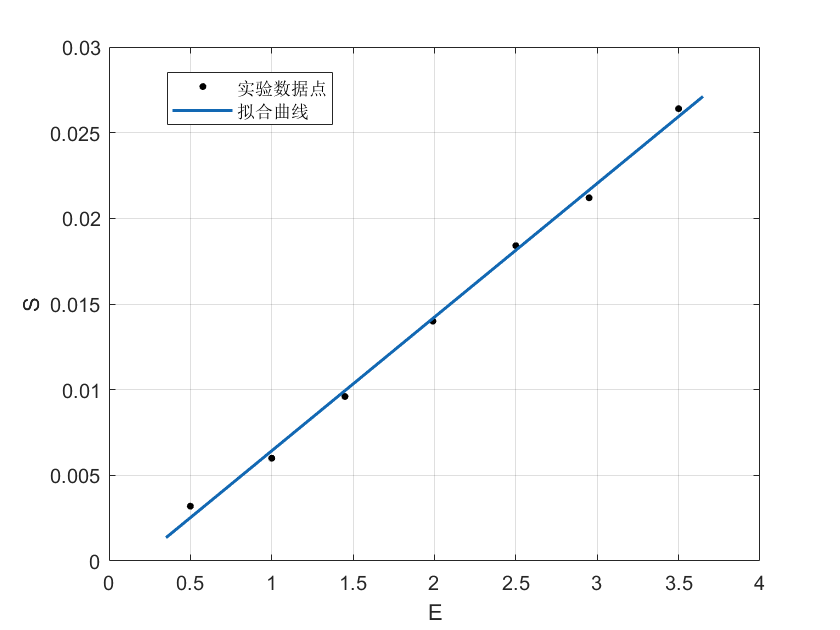
\includegraphics[width=0.8\textwidth]{E-S图}
	\caption{\footnotesize $E-S$图}
\end{figure}
\par 可以看出,$S$与$E$大致呈正比例关系 
\end{document}
